\documentclass{article}
\usepackage{graphicx} % Required for inserting images

\title{COMPSCI 3N03 Assignment 3}
\author{Aditya Sahni, Karan Sandhu, Ankur Pandey, Manavi Manavi }
\date{March 2025}

\begin{document}

\maketitle

\section{Detailed Explanation of the Protocol}

\subsection{Connection Establishment}

The protocol utilizes TCP at the transport layer to guarantee reliable, ordered, and error-free communication between the server and up to four clients. TCP's connection-oriented nature ensures consistency in game state across all participants.

The server initializes a TCP socket, enabling the \texttt{SO\_REUSEADDR} option to allow immediate port reuse. It binds to a user-specified port (e.g., 12345) and begins listening for connections. The server accepts up to four clients, placing each in the \texttt{g\_clientSockets} list, initializing their game state (e.g., position, health), and spawning a dedicated thread (\texttt{clientHandler}) for handling client communication. If the server is at capacity, it sends a message stating the server is full and rejects the connection.

Clients also create TCP sockets and connect using the server's IP and port provided via command-line arguments. Upon a successful connection, the client prints a confirmation message and launches a \texttt{receiverThread} to listen for server updates. The server then broadcasts the current game state to all clients, ensuring the new client starts in sync with the ongoing game.

\subsection{Message Formats and Communication Flow}

The protocol employs UTF-8 encoded, newline-terminated plain-text messages for communication, allowing for straightforward parsing and cross-platform compatibility. Clients issue commands to the server, which responds with game state updates or other notifications.

Clients transmit commands as single-line strings using \texttt{sendall()}, with supported commands as follows:

\begin{itemize}
    \item \textbf{MOVE:} Format: \texttt{MOVE <DIRECTION>} (e.g., \texttt{MOVE UP}). The direction must be one of \texttt{UP}, \texttt{DOWN}, \texttt{LEFT}, or \texttt{RIGHT}.
    \item \textbf{ATTACK:} A single-word command that targets adjacent players.
    \item \textbf{SAY:} Format: \texttt{SAY <MESSAGE>}. Sends a chat message to all players.
    \item \textbf{QUIT:} Signals the client’s intent to disconnect from the server.
\end{itemize}

The server replies with the updated game state to all clients using \texttt{sendall()} on each socket. The message includes:

\begin{itemize}
    \item A header (\texttt{--- GAME STATE ---}).
    \item A 5x5 ASCII grid showing player positions, obstacles, and empty cells.
    \item Player-specific information, including health and coordinates.
    \item Special messages such as ``You have died'' or ``Goodbye!'' where applicable.
\end{itemize}

Additional standalone messages are sent for chat (\texttt{SAY}) and error notifications, each properly terminated for client-side display.

\subsection{Command Handling and Protocol Logic}

The server maintains a global game state in the \texttt{g\_gameState} dictionary, which includes the 5x5 grid, a list of player details (position, health, and status), and the total number of connected clients. To ensure thread safety when multiple clients interact with the game state, a threading lock (\texttt{g\_stateLock}) is employed. This lock prevents race conditions during concurrent state updates.

Command parsing and execution are managed by the \texttt{handleCommand} function, which behaves differently based on the player's current state:

\begin{itemize}
    \item \textbf{MOVE:} The server verifies that the player is alive and active. It calculates the intended new position and validates that it lies within the grid bounds and is not obstructed. If valid, the player’s position is updated.
    
    \item \textbf{ATTACK:} If the player is alive, the server checks all other players for adjacency using Manhattan distance. Any adjacent players lose 20 HP. Those who reach 0 HP are marked inactive, removed from the grid, and sent a “You have died” message.
    
    \item \textbf{SAY:} A chat message is constructed and sent to all active clients. This command does not affect the game state.
    
    \item \textbf{QUIT:} The server sends a “Goodbye!” message to the client, marks the player as inactive, clears their socket entry, reduces the client count, and updates the grid accordingly.
\end{itemize}

After handling each command (excluding \texttt{SAY}), the server refreshes the player positions by removing old markers and updating the grid based on current coordinates. It then broadcasts the updated game state to all clients. Dead players attempting restricted commands receive a “You are now spectating as a ghost...” notification and are limited to using only \texttt{SAY} and \texttt{QUIT}.

\subsection{Error Handling and Robustness}

To enhance reliability, the protocol incorporates comprehensive error handling mechanisms on both the server and client sides. All socket-related operations are enclosed in \texttt{try/except} blocks to capture and respond to exceptions gracefully.

\textbf{On the server side:}

\begin{itemize}
    \item Setup errors such as a port conflict are caught and logged (e.g., “Server setup failed”), prompting a safe exit.
    \item If the maximum number of clients is reached, additional connections are refused with a “Server full” message.
    \item During broadcasts, a \texttt{BrokenPipeError} (e.g., a disconnected client) is logged, and the associated player is marked inactive while the server continues operation.
\end{itemize}

\textbf{On the client side:}

\begin{itemize}
    \item Connection failures result in an immediate exit after displaying an error message.
    \item If no data is received (indicating a disconnect), the socket is closed, and the client exits cleanly.
    \item Sending errors also trigger a safe shutdown of the client.
\end{itemize}

A \texttt{threading.Event} is used to ensure a graceful client shutdown after a \texttt{QUIT} command. The receiving thread is given a short timeout to process the final messages (e.g., “Goodbye!”) before the socket is closed. Players marked as dead are restricted from sending unauthorized commands, maintaining the integrity of the game state.

\subsection{Extensibility and Deployment Considerations}

This protocol is built with adaptability in mind, allowing it to be deployed in multiple environments. During local testing, it uses the loopback address (127.0.0.1) as shown in the quickstart instructions. For LAN-based gameplay, the server binds to all network interfaces (''), enabling clients within the same local network to connect using the server’s LAN IP (e.g., 192.168.1.x), which can be obtained using tools like \texttt{ifconfig} or \texttt{ipconfig}.

For internet-based deployment, further setup is necessary. Specifically, the server's port (e.g., 12345) must be forwarded on the router, and clients must use the server’s public IP or domain name to connect. Because the protocol currently transmits plain-text messages, it is vulnerable to eavesdropping and tampering. To address this, enhancements such as TLS encryption (using Python’s \texttt{ssl} module) and user authentication (e.g., a login feature) could be introduced.

Although the current implementation, which uses a separate thread for each client, handles up to four players efficiently, it can be extended using asynchronous I/O (e.g., \texttt{asyncio}) to support larger player counts. Additionally, new commands like \texttt{HEAL} or \texttt{TRADE} could be incorporated into the \texttt{handleCommand} function. Parameters like \texttt{GRID\_ROWS}, \texttt{GRID\_COLS}, and \texttt{MAX\_CLIENTS} can also be modified to increase the game’s scale, making the protocol highly adaptable for future enhancements.

\subsection{Summary}

The protocol supports a real-time, multiplayer ASCII-based ``Battle Game'' using TCP, emphasizing clarity, reliability, and robustness. Clients send commands such as \texttt{MOVE}, \texttt{ATTACK}, \texttt{SAY}, and \texttt{QUIT}, while the server maintains a synchronized global game state using a dedicated thread for each client and locking mechanisms to prevent data races.

Its comprehensive error-handling approach ensures resilience to network disruptions and disconnections. The architecture allows for both local and LAN-based play, and with added security and scalability features, it could be adapted for online deployment. Overall, the protocol's straightforward and modular design offers a solid basis for expanding multiplayer networked game development.

\section{Sequence Diagram}


\tikzset{every picture/.style={line width=0.75pt}} %set default line width to 0.75pt        

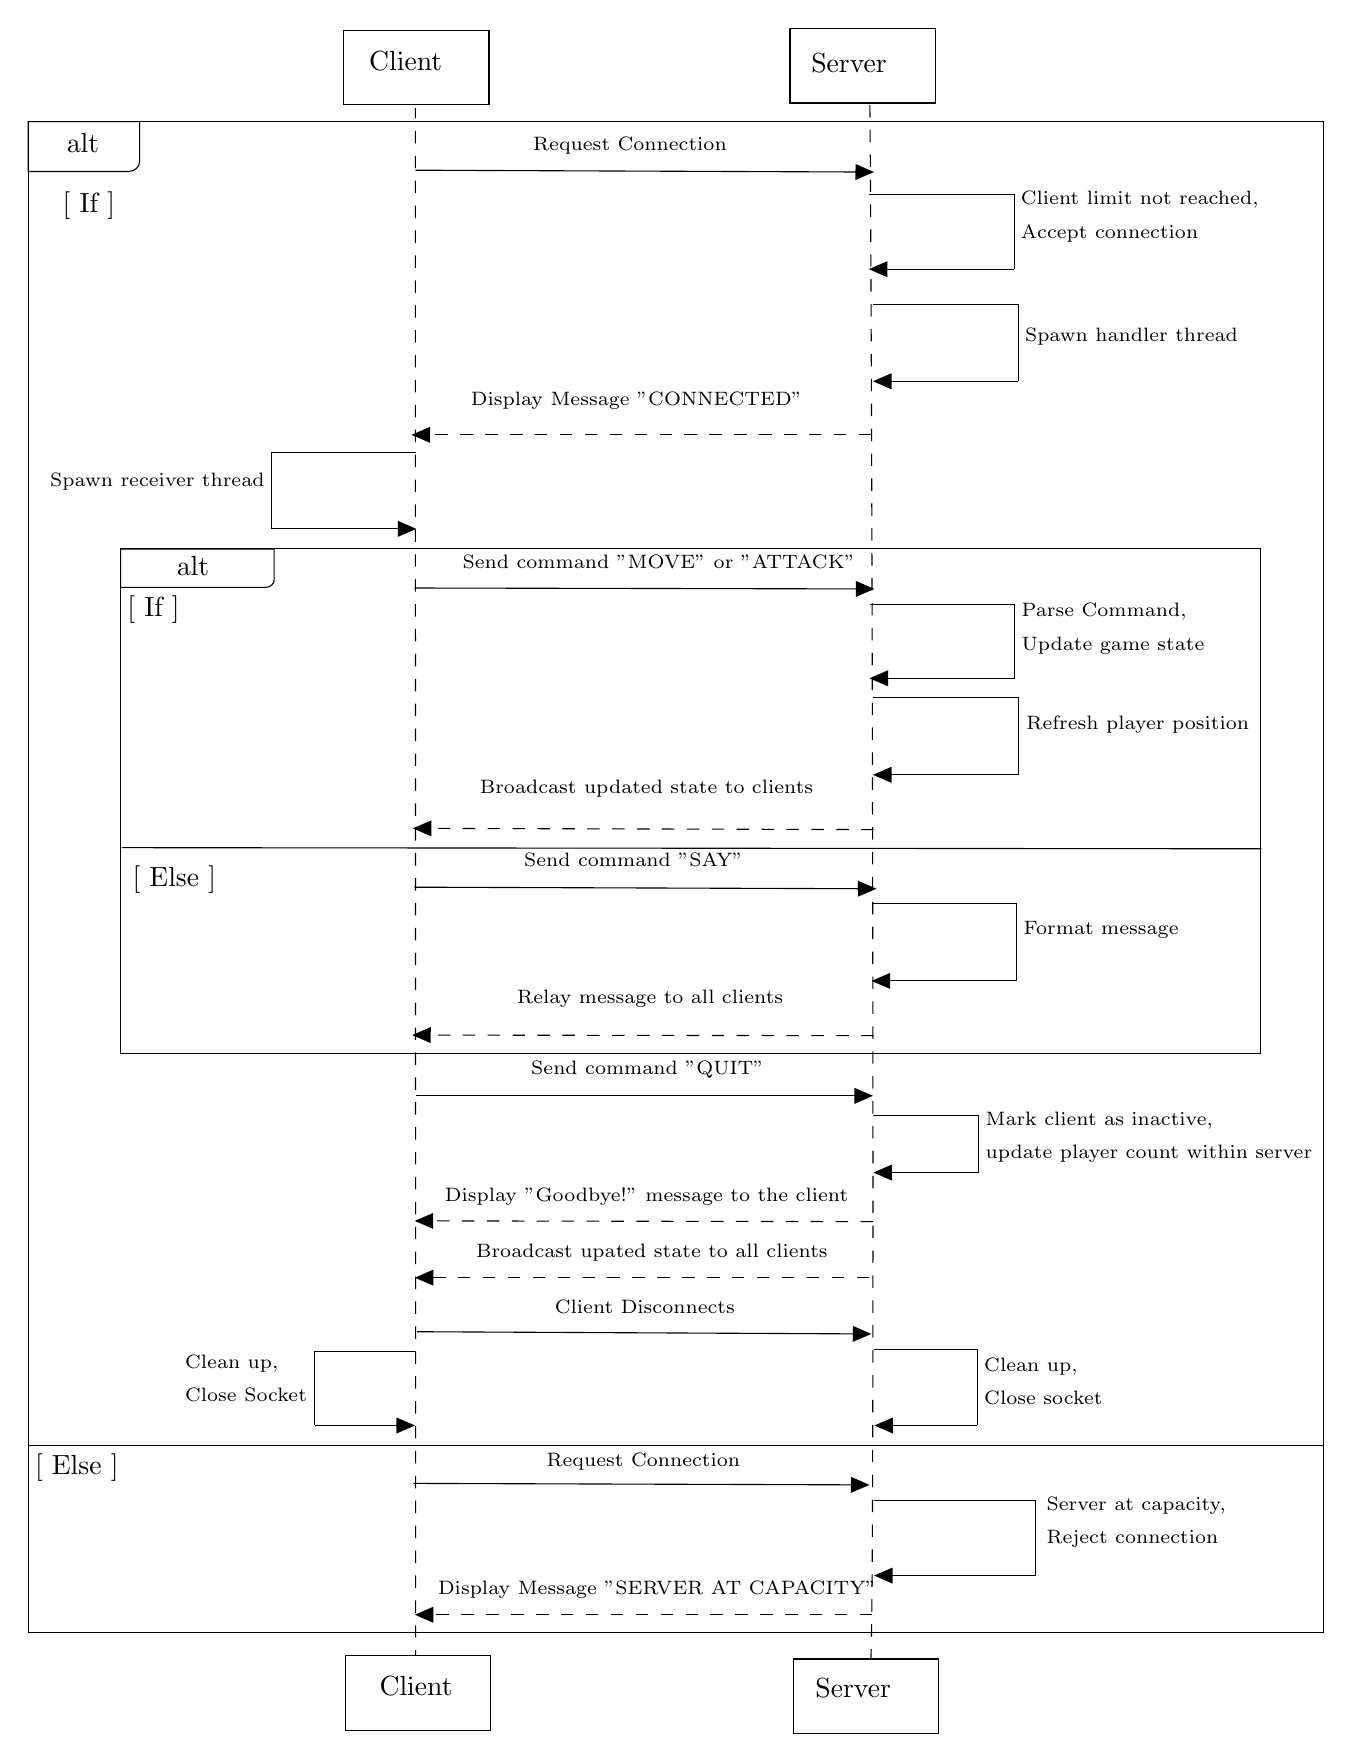
\begin{tikzpicture}[x=0.75pt,y=0.75pt,yscale=-0.9,xscale=1]
%uncomment if require: \path (0,1045); %set diagram left start at 0, and has height of 1045

%Shape: Rectangle [id:dp3086100904245759] 
\draw   (166,13) -- (236,13) -- (236,53) -- (166,53) -- cycle ;
%Shape: Rectangle [id:dp5196240471587756] 
\draw   (381,12) -- (451,12) -- (451,52) -- (381,52) -- cycle ;
%Straight Lines [id:da6385124776961626] 
\draw    (200.5,88) -- (418.5,88.99) ;
\draw [shift={(421.5,89)}, rotate = 180.26] [fill={rgb, 255:red, 0; green, 0; blue, 0 }  ][line width=0.08]  [draw opacity=0] (8.93,-4.29) -- (0,0) -- (8.93,4.29) -- cycle    ;
%Curve Lines [id:da20873191980681205] 
\draw  [dash pattern={on 4.5pt off 4.5pt}]  (200.5,56) .. controls (200.5,16) and (200.67,913) .. (200.67,882) ;
%Curve Lines [id:da4392393233066598] 
\draw  [dash pattern={on 4.5pt off 4.5pt}]  (419.5,53) .. controls (420.5,154) and (422,832.67) .. (420,884.67) ;
%Shape: Right Angle [id:dp4281520430984249] 
\draw   (419,101) -- (489,101) -- (489,141) ;
%Straight Lines [id:da07302771314813206] 
\draw    (489,141) -- (422,141) ;
\draw [shift={(419,141)}, rotate = 360] [fill={rgb, 255:red, 0; green, 0; blue, 0 }  ][line width=0.08]  [draw opacity=0] (8.93,-4.29) -- (0,0) -- (8.93,4.29) -- cycle    ;
%Shape: Right Angle [id:dp09227178846237738] 
\draw   (421,160) -- (491,160) -- (491,201) ;
%Straight Lines [id:da2200355969955725] 
\draw    (491,201) -- (424,201) ;
\draw [shift={(421,201)}, rotate = 360] [fill={rgb, 255:red, 0; green, 0; blue, 0 }  ][line width=0.08]  [draw opacity=0] (8.93,-4.29) -- (0,0) -- (8.93,4.29) -- cycle    ;
%Straight Lines [id:da6257742993511151] 
\draw  [dash pattern={on 4.5pt off 4.5pt}]  (420.17,229.67) -- (201.67,229.67) ;
\draw [shift={(198.67,229.67)}, rotate = 360] [fill={rgb, 255:red, 0; green, 0; blue, 0 }  ][line width=0.08]  [draw opacity=0] (8.93,-4.29) -- (0,0) -- (8.93,4.29) -- cycle    ;
%Shape: Right Angle [id:dp4646986488425606] 
\draw   (201,239) -- (131.33,239) -- (131.33,280) ;
%Straight Lines [id:da3932008336749233] 
\draw    (131.33,280) -- (162.67,280) -- (198,280) ;
\draw [shift={(201,280)}, rotate = 180] [fill={rgb, 255:red, 0; green, 0; blue, 0 }  ][line width=0.08]  [draw opacity=0] (8.93,-4.29) -- (0,0) -- (8.93,4.29) -- cycle    ;
%Straight Lines [id:da07403773160707683] 
\draw    (200.17,311.67) -- (418.67,312.16) ;
\draw [shift={(421.67,312.17)}, rotate = 180.13] [fill={rgb, 255:red, 0; green, 0; blue, 0 }  ][line width=0.08]  [draw opacity=0] (8.93,-4.29) -- (0,0) -- (8.93,4.29) -- cycle    ;
%Shape: Right Angle [id:dp34849832526939095] 
\draw   (419.33,320.5) -- (489.33,320.5) -- (489.33,360) ;
%Straight Lines [id:da14148208217225333] 
\draw    (489.33,360) -- (442.67,360) -- (422.33,360) ;
\draw [shift={(419.33,360)}, rotate = 360] [fill={rgb, 255:red, 0; green, 0; blue, 0 }  ][line width=0.08]  [draw opacity=0] (8.93,-4.29) -- (0,0) -- (8.93,4.29) -- cycle    ;
%Shape: Right Angle [id:dp8734375687405087] 
\draw   (421,370.17) -- (491,370.17) -- (491,411.67) ;
%Straight Lines [id:da4492025030918525] 
\draw    (491,411.67) -- (424,411.67) ;
\draw [shift={(421,411.67)}, rotate = 360] [fill={rgb, 255:red, 0; green, 0; blue, 0 }  ][line width=0.08]  [draw opacity=0] (8.93,-4.29) -- (0,0) -- (8.93,4.29) -- cycle    ;
%Straight Lines [id:da9362318595498027] 
\draw  [dash pattern={on 4.5pt off 4.5pt}]  (421.33,441) -- (341.66,440.76) -- (202.33,440.34) ;
\draw [shift={(199.33,440.33)}, rotate = 0.17] [fill={rgb, 255:red, 0; green, 0; blue, 0 }  ][line width=0.08]  [draw opacity=0] (8.93,-4.29) -- (0,0) -- (8.93,4.29) -- cycle    ;
%Shape: Rectangle [id:dp4186962078189216] 
\draw   (58.5,290.67) -- (607.5,290.67) -- (607.5,561) -- (58.5,561) -- cycle ;
%Straight Lines [id:da7360305644500611] 
\draw    (59.17,450.67) -- (608.07,451.27) ;
%Rounded Single Corner Rect [id:dp0574911480161262] 
\draw   (132.5,307.23) .. controls (132.5,309.5) and (130.66,311.33) .. (128.4,311.33) -- (58.5,311.33) -- (58.5,290.83) -- (132.5,290.83) -- cycle ;
%Straight Lines [id:da911582935971557] 
\draw    (200,471.83) -- (419.67,472.66) ;
\draw [shift={(422.67,472.67)}, rotate = 180.21] [fill={rgb, 255:red, 0; green, 0; blue, 0 }  ][line width=0.08]  [draw opacity=0] (8.93,-4.29) -- (0,0) -- (8.93,4.29) -- cycle    ;
%Shape: Right Angle [id:dp8329913269010942] 
\draw   (420.33,480.67) -- (490.33,480.67) -- (490.33,522) ;
%Straight Lines [id:da3987289645810945] 
\draw    (490.33,522) -- (423.33,522) ;
\draw [shift={(420.33,522)}, rotate = 360] [fill={rgb, 255:red, 0; green, 0; blue, 0 }  ][line width=0.08]  [draw opacity=0] (8.93,-4.29) -- (0,0) -- (8.93,4.29) -- cycle    ;
%Straight Lines [id:da777619853671264] 
\draw  [dash pattern={on 4.5pt off 4.5pt}]  (421.33,551.33) -- (202,551) ;
\draw [shift={(199,551)}, rotate = 0.09] [fill={rgb, 255:red, 0; green, 0; blue, 0 }  ][line width=0.08]  [draw opacity=0] (8.93,-4.29) -- (0,0) -- (8.93,4.29) -- cycle    ;
%Straight Lines [id:da6404404065746214] 
\draw    (200.6,583.53) -- (418,583.53) ;
\draw [shift={(421,583.53)}, rotate = 180] [fill={rgb, 255:red, 0; green, 0; blue, 0 }  ][line width=0.08]  [draw opacity=0] (8.93,-4.29) -- (0,0) -- (8.93,4.29) -- cycle    ;
%Shape: Right Angle [id:dp7663465839213492] 
\draw   (421.2,594.2) -- (471.8,594.2) -- (471.8,624.6) ;
%Straight Lines [id:da24096355138571712] 
\draw    (471.8,624.6) -- (424.2,624.6) ;
\draw [shift={(421.2,624.6)}, rotate = 360] [fill={rgb, 255:red, 0; green, 0; blue, 0 }  ][line width=0.08]  [draw opacity=0] (8.93,-4.29) -- (0,0) -- (8.93,4.29) -- cycle    ;
%Straight Lines [id:da4090529486102783] 
\draw  [dash pattern={on 4.5pt off 4.5pt}]  (421,650.87) -- (203.2,650.47) ;
\draw [shift={(200.2,650.47)}, rotate = 0.1] [fill={rgb, 255:red, 0; green, 0; blue, 0 }  ][line width=0.08]  [draw opacity=0] (8.93,-4.29) -- (0,0) -- (8.93,4.29) -- cycle    ;
%Straight Lines [id:da5293640230132644] 
\draw  [dash pattern={on 4.5pt off 4.5pt}]  (419.07,680.87) -- (203.27,680.87) ;
\draw [shift={(200.27,680.87)}, rotate = 360] [fill={rgb, 255:red, 0; green, 0; blue, 0 }  ][line width=0.08]  [draw opacity=0] (8.93,-4.29) -- (0,0) -- (8.93,4.29) -- cycle    ;
%Straight Lines [id:da8126720732231536] 
\draw    (201.4,709.8) -- (417.2,710.98) ;
\draw [shift={(420.2,711)}, rotate = 180.31] [fill={rgb, 255:red, 0; green, 0; blue, 0 }  ][line width=0.08]  [draw opacity=0] (8.93,-4.29) -- (0,0) -- (8.93,4.29) -- cycle    ;
%Shape: Right Angle [id:dp42352922413277505] 
\draw   (200.33,720.33) -- (152,720.33) -- (152,760) ;
%Shape: Right Angle [id:dp04860851042037817] 
\draw   (421.67,719.33) -- (471.33,719.33) -- (471.33,760) ;
%Straight Lines [id:da5036428196951162] 
\draw    (152,760) -- (197.33,760) ;
\draw [shift={(200.33,760)}, rotate = 180] [fill={rgb, 255:red, 0; green, 0; blue, 0 }  ][line width=0.08]  [draw opacity=0] (8.93,-4.29) -- (0,0) -- (8.93,4.29) -- cycle    ;
%Straight Lines [id:da9536494516623164] 
\draw    (471.33,760) -- (424.67,760) ;
\draw [shift={(421.67,760)}, rotate = 360] [fill={rgb, 255:red, 0; green, 0; blue, 0 }  ][line width=0.08]  [draw opacity=0] (8.93,-4.29) -- (0,0) -- (8.93,4.29) -- cycle    ;
%Shape: Rectangle [id:dp6192774424375358] 
\draw   (14,62) -- (638,62) -- (638,870.67) -- (14,870.67) -- cycle ;
%Rounded Single Corner Rect [id:dp727473675653419] 
\draw   (67.67,83.33) .. controls (67.67,86.28) and (65.28,88.67) .. (62.33,88.67) -- (14,88.67) -- (14,62) -- (67.67,62) -- cycle ;
%Straight Lines [id:da0436318807502325] 
\draw    (14,770.67) -- (638,770.67) ;
%Straight Lines [id:da335861472962917] 
\draw    (199.73,791) -- (416.33,791.79) ;
\draw [shift={(419.33,791.8)}, rotate = 180.21] [fill={rgb, 255:red, 0; green, 0; blue, 0 }  ][line width=0.08]  [draw opacity=0] (8.93,-4.29) -- (0,0) -- (8.93,4.29) -- cycle    ;
%Shape: Right Angle [id:dp5438923416054762] 
\draw   (421.53,800.33) -- (499.33,800.33) -- (499.33,840.33) ;
%Straight Lines [id:da8536553031123704] 
\draw    (499.33,840.33) -- (424.53,840.33) ;
\draw [shift={(421.53,840.33)}, rotate = 360] [fill={rgb, 255:red, 0; green, 0; blue, 0 }  ][line width=0.08]  [draw opacity=0] (8.93,-4.29) -- (0,0) -- (8.93,4.29) -- cycle    ;
%Straight Lines [id:da978168065075302] 
\draw  [dash pattern={on 4.5pt off 4.5pt}]  (420.67,861.33) -- (203.27,861.33) ;
\draw [shift={(200.27,861.33)}, rotate = 360] [fill={rgb, 255:red, 0; green, 0; blue, 0 }  ][line width=0.08]  [draw opacity=0] (8.93,-4.29) -- (0,0) -- (8.93,4.29) -- cycle    ;
%Shape: Rectangle [id:dp9923763921681099] 
\draw   (166.67,883.33) -- (236.67,883.33) -- (236.67,923.33) -- (166.67,923.33) -- cycle ;
%Shape: Rectangle [id:dp9528472722825438] 
\draw   (382.67,885) -- (452.67,885) -- (452.67,925) -- (382.67,925) -- cycle ;

% Text Node
\draw (177,23) node [anchor=north west][inner sep=0.75pt]   [align=left] {Client};
% Text Node
\draw (390,24) node [anchor=north west][inner sep=0.75pt]   [align=left] {Server};
% Text Node
\draw (256,69) node [anchor=north west][inner sep=0.75pt]   [align=left] {{\scriptsize Request Connection}};
% Text Node
\draw (491,98) node [anchor=north west][inner sep=0.75pt]   [align=left] {{\scriptsize Client limit not reached,}\\{\scriptsize Accept connection}};
% Text Node
\draw (493,171) node [anchor=north west][inner sep=0.75pt]   [align=left] {{\scriptsize Spawn handler thread}};
% Text Node
\draw (226,205.33) node [anchor=north west][inner sep=0.75pt]   [align=left] {{\scriptsize Display Message "CONNECTED"}};
% Text Node
\draw (23.33,248.5) node [anchor=north west][inner sep=0.75pt]   [align=left] {{\scriptsize Spawn receiver thread}};
% Text Node
\draw (222,292.67) node [anchor=north west][inner sep=0.75pt]   [align=left] {{\scriptsize Send command "MOVE" or "ATTACK"}};
% Text Node
\draw (491.33,318.5) node [anchor=north west][inner sep=0.75pt]   [align=left] {{\scriptsize Parse Command,}\\{\scriptsize Update game state}};
% Text Node
\draw (493.67,378.83) node [anchor=north west][inner sep=0.75pt]   [align=left] {{\scriptsize Refresh player position}};
% Text Node
\draw (230.33,413.33) node [anchor=north west][inner sep=0.75pt]   [align=left] {{\scriptsize Broadcast updated state to clients}};
% Text Node
\draw (84.33,293.17) node [anchor=north west][inner sep=0.75pt]   [align=left] {alt};
% Text Node
\draw (60.5,314.33) node [anchor=north west][inner sep=0.75pt]   [align=left] {[ If ]};
% Text Node
\draw (63,459.17) node [anchor=north west][inner sep=0.75pt]   [align=left] {[ Else ]};
% Text Node
\draw (251.67,452.33) node [anchor=north west][inner sep=0.75pt]   [align=left] {{\scriptsize Send command "SAY"}};
% Text Node
\draw (492.33,488.67) node [anchor=north west][inner sep=0.75pt]   [align=left] {{\scriptsize Format message}};
% Text Node
\draw (248.33,525.67) node [anchor=north west][inner sep=0.75pt]   [align=left] {{\scriptsize Relay message to all clients}};
% Text Node
\draw (255.07,563.73) node [anchor=north west][inner sep=0.75pt]   [align=left] {{\scriptsize Send command "QUIT"}};
% Text Node
\draw (474,590.6) node [anchor=north west][inner sep=0.75pt]   [align=left] {{\scriptsize Mark client as inactive,}\\{\scriptsize update player count within server}};
% Text Node
\draw (213.47,631.4) node [anchor=north west][inner sep=0.75pt]   [align=left] {{\scriptsize Display "Goodbye!" message to the client }};
% Text Node
\draw (228.53,661.27) node [anchor=north west][inner sep=0.75pt]   [align=left] {{\scriptsize Broadcast upated state to all clients}};
% Text Node
\draw (266.47,691.4) node [anchor=north west][inner sep=0.75pt]   [align=left] {{\scriptsize Client Disconnects}};
% Text Node
\draw (88.33,720.67) node [anchor=north west][inner sep=0.75pt]   [align=left] {{\scriptsize Clean up,}\\{\scriptsize Close Socket}};
% Text Node
\draw (473.33,722.33) node [anchor=north west][inner sep=0.75pt]   [align=left] {{\scriptsize Clean up,}\\{\scriptsize Close socket}};
% Text Node
\draw (31.33,67) node [anchor=north west][inner sep=0.75pt]   [align=left] {alt};
% Text Node
\draw (29.33,98) node [anchor=north west][inner sep=0.75pt]   [align=left] {[ If ]};
% Text Node
\draw (16,773.67) node [anchor=north west][inner sep=0.75pt]   [align=left] {[ Else ]};
% Text Node
\draw (262.47,773.47) node [anchor=north west][inner sep=0.75pt]   [align=left] {{\scriptsize Request Connection}};
% Text Node
\draw (503.4,797.13) node [anchor=north west][inner sep=0.75pt]   [align=left] {{\scriptsize Server at capacity,}\\{\scriptsize Reject connection}\\};
% Text Node
\draw (210.2,841.87) node [anchor=north west][inner sep=0.75pt]   [align=left] {{\scriptsize Display Message "SERVER AT CAPACITY"}};
% Text Node
\draw (182,892.67) node [anchor=north west][inner sep=0.75pt]   [align=left] {Client};
% Text Node
\draw (392,894.33) node [anchor=north west][inner sep=0.75pt]   [align=left] {Server};


\end{tikzpicture}

\end{document}
